\section{\SYSTEM{}: Learning Control}
\label{sec:framework}

\begin{figure}
  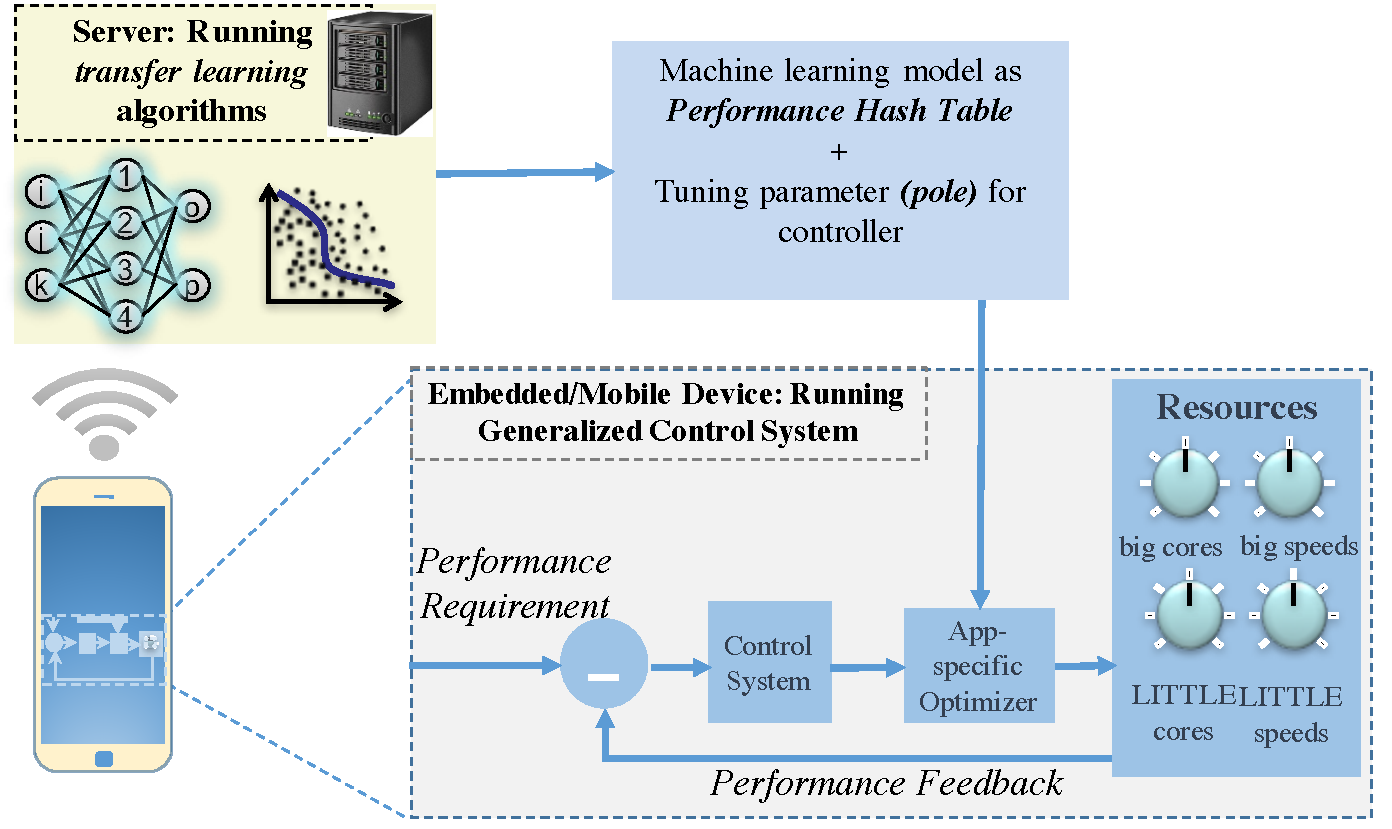
\includegraphics[width=\columnwidth]{figures/Overview.pdf}
  \caption{\SYSTEM{} overview.}
  \label{fig:overview}
\end{figure}


We describe \SYSTEM{}'s parameter-free resource management system,
which assumes no prior knowledge of the application and requires no
user-specified parameters.  \figref{fig:overview} shows \SYSTEM{}'s
approach.  A new application enters the system with a performance
requirement.  A generalized adaptive control system allocates
resources according to a generic model and records performance and
power.  The recorded values are sent to a learner, which estimates the
application's performance and power in all other configurations and
extracts those that represent Pareto-optimal tradeoffs.  These
configurations are packaged in a special data structure---the
performance hash table (PHT).  The learner sends the PHT, the
estimated variance, and a confidence interval to the controller.
Using these values, the controller selects an energy minimal resource
configuration in constant time with formal guarantees that it will
converge to the desired performance.

\begin{figure}
  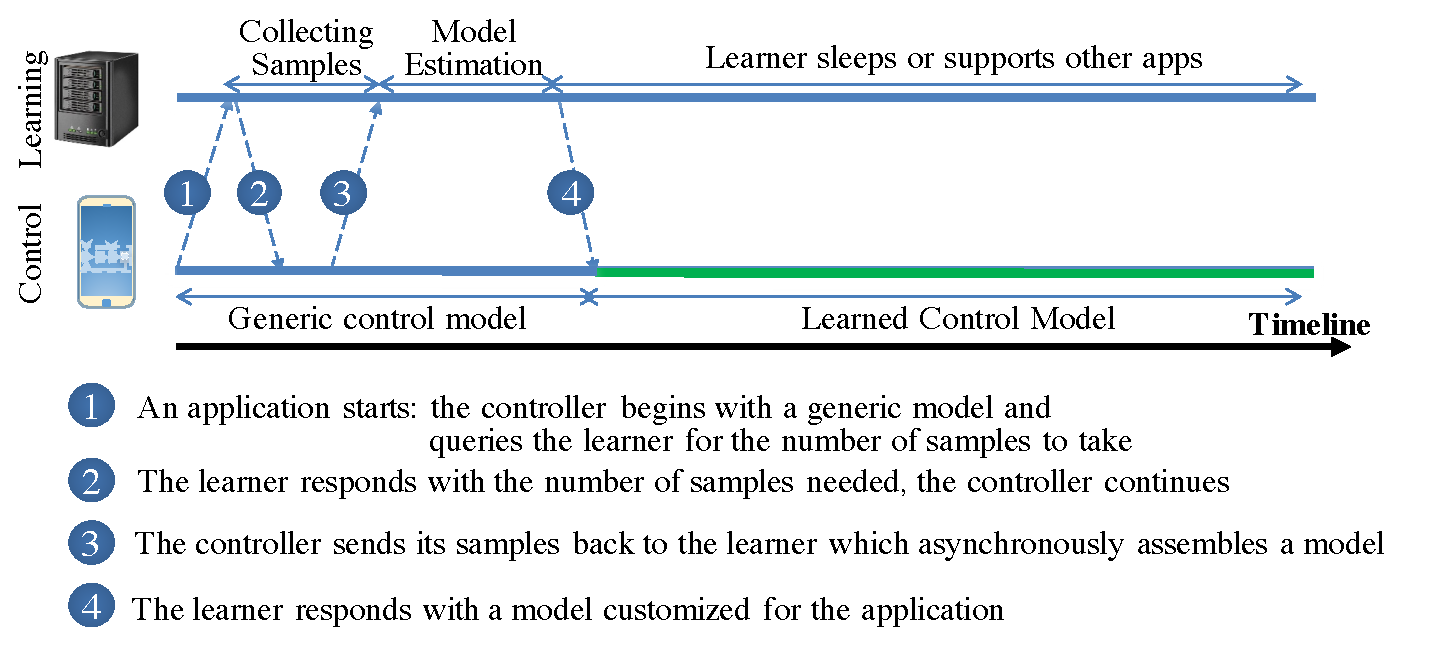
\includegraphics[width=\columnwidth]{figures/Timeline.pdf}
  \caption{Temporal relationship of the learning and control system.}
  \label{fig:timeline}
\end{figure}

\figref{fig:timeline} illustrates the asynchronous interaction between
\SYSTEM{}'s learner and controller over time. The controller starts
when a new application launches.  Since the controller has no prior
knowledge of this application, it begins allocating resources using a
generic model.  At application launch, the controller sends the
learner the application name and device type (message 1,
\figref{fig:timeline}).  The learner determines how many samples are
needed for an accurate estimate and sends this number back to the
controller (message 2).  The controller takes these samples while
using the generic model and sends the learner a message with the
performance and power of each measured configuration (message 3).
Computationally expensive learners may require some time to build a
model from these observations.  The controller does not wait for the
learner, but contiues with the generic model.  Once the learner has a
model and variance estimate, it sends that data to the controller
(message 4). From then on, the controller uses the learned model.

\figref{fig:timeline} shows several key points about the relationship
between learning and control.  First, the controller never waits for
the learner---it uses a generic model to provide less efficient
control until the learner can produce a customized model. Second, the
controller does not continuously communicate with the learner, this
interaction happens once at application launch.  Third, if the learner
crashed, the controller would just default to the behavior of a
generic adaptive control system.  If the learner crashed after
producing a model, control might not even need to know.  Finally,
because the learner and controller have a clearly defined interface,
they can be run in separate processes or physically separate devices.

This section first describes a traditional adaptive control system
designed for a heterogeneous processor.  We then generalize this
approach and separate out parameters to be learned.  Next, we discuss
the general class of learning systems that can work with \SYSTEM{}.
Then, we present an encoding for the learned model that can be
accessed by the controller in constant time.  Finally, we analyze
\SYSTEM{}'s formal guarantees.


\subsection{Traditional Control for Computing}
Several researchers have proposed controlling computing systems.  A
controller that can manage multiple resources to meet multiple goals
is a multiple-input, multiple-output (MIMO) controller.  The inputs
are measurements, \eg{} performance.  The outputs are the resource
settings to be used at a particular time, \eg{} an allocation of big
and LITTLE cores and a clockspeed for each.

The following difference equations describe a generic MIMO controller
for allocating $n$ resources to meet $m$ goals at time
$t$:\footnote{We assume discrete time, and thus, use difference
  equations rather than differential equations that would be used for
  continuous systems.}
\begin{equation}
\begin{aligned}
&\x(t+1) &=& \mathbf{A} \cdot \x(t)& + \mathbf{B} \cdot \mathbf{c}(t)\\
&\y(t)   &=& \mathbf{C} \cdot \x(t)&,
\end{aligned}
\label{eqn:system:mimo}
\end{equation}
where $\x \in \R^{q}$ is the controller's \emph{state}, an abstract
representation of the relationship between resources and goals.
$\mathbf{c}(t) \in \R^n$ is a vector representing the current
\emph{configuration} of resources; \ie{} the $i$th vector element
represents the amount of resource $i$ to be allocated at time $t$.
$\y(t) \in \R^{m}$ represents the current value of the goal dimensions
at time $t$. The matrices $\mathbf{A} \in \R^{q \times q}$ and
$\mathbf{B} \in \R^{q \times n}$ relate the resource configuration to
the controller state.  The matrix $\mathbf{C} \in \R^{m \times q}$
relates the controller state to the expected behavior.  This model
does not assume the states or the resources are independent, but it
does assume that their relationship is linear.

For example, to allocate resources to meet performance goals in our
ARM big.LITTLE system---from \secref{example}---there are four
resources: the number of big cores, the number of LITTLE cores, and
the speeds for each of the big and LITTLE cores.  There is also a
single goal: performance.  Thus, in this example, $n=4$ and $m=1$. The
vector $\mathbf{c}(t)$ has four elements representing the resource
allocation at time $t$.  The matrices $\mathbf{A}$, $\mathbf{B}$, and
$\mathbf{C}$ capture the linear relationship between the control state
$\x$, the resource usage $\mathbf{c}$, and the measured behavior.  In
this example, we know there is a non-linear relationship between the
resources.  We overcome this difficulty by tuning the identified
matrices at each time step---approximating the non-linear system
through a series of changing linear formulations.  This approximation
is a form of \emph{adaptive} or \emph{self-tuning} control
\cite{AdaptiveControl}.  Such adaptive controllers provide formal
guarantees that they will converge to the desired performance even in
the face of non-linearities, but they still assume convexity.

This control formulation has two major drawbacks.  First, because it
requires matrix computation, its overhead scales linearly in the
number of resources and in the number of goals
\cite{Hellerstein2004a,METE}.  Second, the adaptive mechanisms are not
parameter-free---they require users to specify starting values of the
matrices $\mathbf{A}$, $\mathbf{B}$, and $\mathbf{C}$ and the method
for updating these matrices to account for any non-convexity in the
relationship between resources and performance
\cite{POET,METE,ControlWare,AdaptiveControl}.  Therefore, typically
100s to 1000s of samples are taken when the controller is designed to
ensure that the starting matrices are sufficient to prevent the
controller from getting stuck in a local optima
\cite{FSE2015,sysid,josep-isca2016}.

\subsection{\SYSTEM{} Control System}
To overcome the above issues, \SYSTEM{} abstracts the controller of
\eqnref{system:mimo} and factors out those parameter to be learned.
Specifically, \SYSTEM{} takes three steps to transform a standard
control system into one that works without prior knowledge of the
application to be controlled:
\begin{enumerate}[leftmargin=1em]
\item controlling \emph{speedup} rather than resources,
\item translating speedup into an energy minimal \emph{resource
    schedule} in a separate step, and
\item exploiting the \emph{problem structure} to solve this scheduling
  problem in constant time.
\end{enumerate}
These steps assume a separate learner has produced a model of resource
performance and power.  The result is that \SYSTEM{}'s controller runs
in constant time without requiring any user-specified parameters.


% We first describe our formulation for controlling speedup and then
% converting that speedup into resource allocations.

\subsubsection{Controlling Speedup}
Instead of the matrix equations of \eqnref{system:mimo}, \SYSTEM{}
uses a scalar difference model relating speedup to performance:
\begin{equation}
  perf(t) = b(t) \cdot speedup(t-1) + \delta \label{eqn:speedup}
\end{equation}
where $b(t)$ is the application's \emph{base speed}: defined as the
speed when all resources are available.  While $b(t)$ is application
specific, it is easy to measure online, by simply allocating all
resources. Such a configuration should not violate any performance
constraints (although it is unlikely to be energy efficient) so it is
safe to take this measurement.  \SYSTEM{} assumes base speed is
time-variant as applications will transition through phases.

With this model, \SYSTEM{}'s control law is simply:
\begin{eqnarray}
  error(t) &=& goal - perf(t) \label{eqn:speedup-error} \\
  % speedup(t) &=& speedup(t-1) - \frac{error(t)}{b}
  speedup(t) &=& speedup(t-1) - \frac{1 - \rho(t)}{b(t)}.error(t)
  \label{eqn:speedup-control}
\end{eqnarray}
which states that the speedup at time $t$ is a function of the
previous speedup, the error at time $t$, the base speed $b(t)$, and
the controller's \emph{pole} $rho(t)$.  Standard control techniques
statically determine the pole and the base speed, but \SYSTEM{}
\emph{dynamically sets the pole and base speed to account for error in
  the learned models---an essential modification for providing formal
  guarantees of the combined control and learning systems.}  For
stable control, \SYSTEM{} ensures $0 \le $rho(t)$ < 1$. Small values
of $\rho(t)$ eliminate error quickly, but make the controller more
sensitive to model inaccuracies.  Larger $\rho(t)$ makes the system
more robust at the cost of reduced convergence time.  \SYSTEM{} sets
$b(t)$ using the standard technique of Kalman filter estimation
\cite{whelch2006kalman}. We describe how \SYSTEM{} automatically sets
the pole in \secref{guarantees}.  First, however, we address the
problem of converting an abstract speedup into a resource allocation.

\subsubsection{Converting Speedup to Resource Schedules}
\SYSTEM{} must map \eqnref{speedup-control}'s speedup into a resource
allocation.  On our example ARM big.LITTLE architecture that means
mapping speedup into an allocation of big and LITTLE cores as well as
a speed for both (big and LITTLE cores are in separate clock domains).

The primary challenge is that speedups in real systems are discrete
non-linear functions of resource usage, while \eqnref{speedup-control}
is a continuous linear function.  We bridge this divide by assigning
time to resource allocations such that the average speedup over a
control interval is that produced by \eqnref{speedup-control}.

We call the assignment of times to resource configurations a
\emph{schedule}. For example, spending 10 ms on the LITTLE cores at
0.6 GHz and then 15 ms on the big cores at 1 GHz is a schedule. There
are typically many schedules that deliver a particular speedup and
\SYSTEM{} must find one with minimal energy.  Given a time interval
$T$, the $speedup(t)$ from \eqnref{speedup-control}, and $C$ different
resource configurations, \SYSTEM{} solves:
\begin{eqnarray}
  \minimize_{\mathbf{\tau} \in \R^{C}} && \sum_{c=0}^{C-1} \tau_c \cdot p_c \label{eqn:power}  \\
  \st %&& \nonumber\\
  && \sum_{c=0}^{C-1} \tau_c \cdot s_c =  speedup(t)T \label{eqn:work} \\
  && \sum_{c=0}^{C-1} \tau_c =  T \label{eqn:deadline} \\
  && 0 \le \tau_c \le T, \qquad \forall c \in \{0,\ldots,C-1\} \label{eqn:time}
\end{eqnarray}
where $p_c$ and $s_c$ are configuration $c$'s estimated
\emph{powerup}---analogous to speedup---and speedup; $\tau_c$ is the
time to spend in configuration $c$.  \eqnref{power} is the objective:
minimizing energy (power times time).  \eqnref{work} states that the
average speedup must be maintained, while \eqnref{deadline} requires
the time to be fully utilized.  \eqnref{time} simply avoids negative
time.

\subsection{Exploiting Structure for Fast Solutions}
%\SYSTEM{} solves \eqnrref{power}{time} on the local device (see
%\figref{fig:timeline}, so the solution must be efficient.  
By expoiting the problem structure and encoding the learned model in
the performance hash table (PHT), \SYSTEM{} solves
\eqnrref{power}{time} in constant ($O(1)$) time.

Kim et al. analyze solutions to the problem of minimizing energy while
meeting a performance constraint and observe that there must be an
optimal solution with the following properties \cite{kim-cpsna}:
\begin{itemize}[leftmargin=1em]
\item At most two of $\tau_c$ are non-zero, meaning that at most two
  configurations will be used in any time interval.
\item If you chart the configurations in the power and performance
  tradeoff space (\eg{} the top half of \figref{fig:pht}) the two
  configurations with non-zero $\tau_c$ lie on the lower convex hull
  of the power performance tradeoff space.
\end{itemize}
%\SYSTEM{} uses these two facts to construct a constant time algorithm
%for finding the optimal solution online.

\begin{figure}
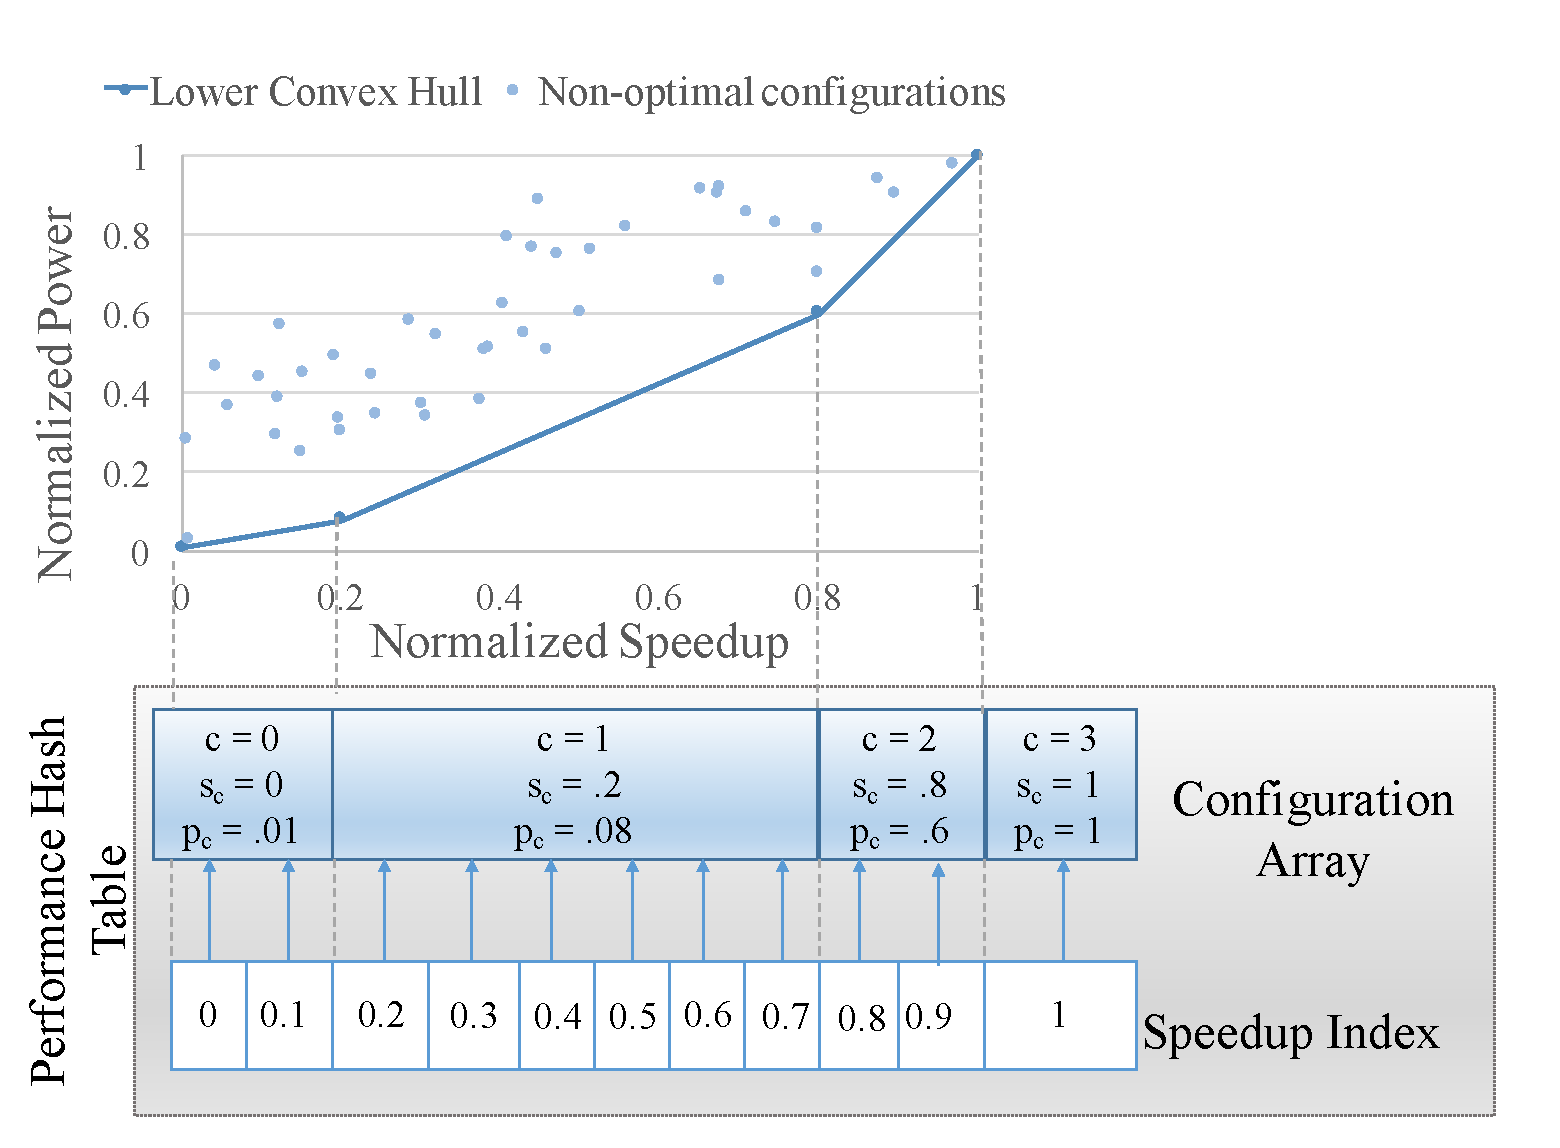
\includegraphics[width=\columnwidth]{figures/performance-hash-table.pdf}
\caption{Data structure to efficiently convert required speedup into a
  resource configuration.}
  \label{fig:pht}
\end{figure}

The PHT (shown in \figref{fig:pht}) provides constant time access to
points on the lower convex hull.  It consists of two arrays: the first
being pointers into the second, which stores resource configurations
on the lower convex hull sorted by speedup.  Recall speedups are
computed relative to the base speed, which uses all resources.  The
largest estimated speedup is therefore 1, so \SYSTEM{} needs only
consider speedups between 0 and 1.  The first array of pointers has a
\emph{resolution} indicating how many decimal points of precision it
captures and it is indexed by speedup.  The example in
\figref{fig:pht} has a resolution of $0.1$.  Each pointer in the first
array points to the configuration in the second array that has the
largest speedup less than or equal to the index.

\SYSTEM{} computes $speedup(t)$ and uses the PHT to convert speedup
into two configurations referred to as $hi$ and $lo$.  To find the
$hi$ configuration, the translator clamps the desired speedup to the
largest index lower than $speedup(t)$ and then walks forward until it
finds the first configuration with a speedup higher than $speedup(t)$.
To find the $lo$ configuration, the translator clamps the desired
speedup to the smallest index higher than $speedup(t)$ and then walks
backwards until it finds the configuration with the largest speedup
less than $speedup(t)$.

For example, consider the PHT in \figref{fig:pht} and an optimizer
meeting $speedup(t) = .65$.  To find $hi$, the optimizer indexes at .6
and walks up to find $c=2$ with $s_c=.8$, setting $hi = 2$.  To find
$lo$, the optimizer indexes the table at .7 and walks backward to find
$c=1$ with $s_c=.2$, setting $lo = 1$.

\SYSTEM{} sets $\tau_{hi}$ and $\tau_{lo}$ by solving:
\begin{eqnarray}
  T &=& \tau_{hi} + \tau_{lo}    \label{eqn:s1} \\
  speedup(t) &=& \frac{s_{hi} \cdot \tau_{hi} + s_{lo} \cdot \tau_{lo}}{T} \label{eqn:s2}
\end{eqnarray}
where $speedup(t)$ is given by the controller and $s_c$ are speedups
estimated by the learner.  By solving \eqnsref{s1}{s2}, \SYSTEM{} has
turned the controller's speedup into a schedule of resource
allocations using learned models stored in the PHT.

\subsection{\SYSTEM{} Learning Algorithms}
The previous subsection describes a general control system, which can
be customized with a number of different learning methods.  The
requirements on the learner are that it must produce 1) estimates of
the speedup and powerup values for each resource configuration and 2)
an estimate of its own inaccuracy.
% We also provide a proxy for self tuning parameter in the later
% sections in case the learning algorithm cannot provide the
% confidence interval.
This section describes the general class of learning mechanisms that
meet these requirements. 

When selecting a learning framework we must find a tradeoff between
the specific and the general; \ie between frameworks that build
application-specific models and frameworks that combine observations
across applications.  For example, the key to energy efficiency on
heterogeneous mobile systems is knowing when to make use of the
smaller, low-power cores \cite{}.  An application-specific model will
capture that precisely, but may require many observations before
producing the correct model.  A more general model will capture the
trend, \eg when most applications should transition, but this general
model might miss the key inflection point for some applications.  We
refer to application-specific models as \emph{online} because they
build models for the current application and do not incorporate
knowledge of other applications.  We refer to general models as
\emph{offline} as they use prior observations of other applications to
predict the behavior of a new application. A third class of
\emph{transfer learning} models combines information from the
previously seen applications and current application to make the
predictions on the application in hand. \TODO{I am assuming it is okay
  to refer to this third class as transfer learning.  IF so, we need a
  citation.}

% The HBM provides a good balance between the online and offline
% approaches.  A strictly online approach will handle each new
% application completely separately and ignore observations of previous
% applications.  This approach never risks contaminating a model with
% unrelated observations, but it may take many observations of the
% current application to converge because it starts with no prior
% knowledge. The offline approach uses all observations from prior
% applications and will therefore converge very quickly; however, it is
% overly general and cannot learn features specific to a single
% application.

\subsubsection{Regression models}
\TODO{Is this offline or online or both?  The prior paragraph sets up
  this three-legged structure: offline, online, and something which we
  used to call hybrid but sounds like we are now calling transfer
  learning. If we are going to keep that structure we should mimic it
  in the substructure of the rest of the section.}  In general, all
machine learning techniques take observations of some phenomena and
produce a model to estimate future outcomes.  In our specific case, we
want to take observations about application's performance and power
given a resource allocation and predict future applications' behavior.
The most straightforward approach is to create a linear regression
model based on the configuration laid out as the input features
\cite{}. Learning in this model requires samples of the performance
and power for different resource configurations. Since the systems are
usually non-linear, polynomial regression models often give better
results, but increase the number of samples required to fit the model
\cite{}. Regression models provide a confidence interval for their
estimates which is important for adaptively tuning the pole.

\subsubsection{Transfer learning}

Another interesting construction is \textit{transfer learning}; which
means we apply the knowledge gained from one scenario to a new,
similar problem.  To provide intuition we offer a simple example.
Suppose we have observed many prior applications, all of which are
either completely compute-bound or completely memory-bound, and we
have an equal number of both.  The only resource we can allocate is
clockspeed, which will increase the performance of compute-bound
applications, but not memory-bound ones.  When we encounter new
application, we must estimate its response to clockspeed.  The online
model will not use prior knowledge, but will observe many different
clock speeds for the new application, leading to high overhead.  The
offline model will predict the mean response of prior applications,
meaning it will over-allocate speed to memory-bound applications and
under-allocate to compute-bound ones.  The transfer learning approach
takes a small number of samples and combines those with prior
knowledge: if the new observations show that clockspeed has no effect
on performance these models will use only the prior memory bound
applications, otherwise, it will use the compute-bound applications.

\paragraph{Netflix Algorithm:}
The Netflix problem is a famous challenge posted by Netflix to find
estimate users' movie preferences. The challenge was one by realizing
that if 2 users both like some movies they might have similar taste in
other movies. This approach allows allows models to borrow large
amounts of data from other users to answer some questions about a new
user.  
%One of the solutions in designing this mathematically is to say
%the the matrix of users vs movies is low rank and solve the problem
%using mathematical optimization techniques.
Delemitriou and Kozyrakis use this algorithm to predict application
response to heterogeneous resources in data centers\cite{Paragon}.


\paragraph{ Bayesian Models:} A hierarchical Bayesian model (HBM)
provides a statistically sound framework for learning across
applications and devices \cite{LEO}.  In this approach, each
application has its own model, allowing specificity, but these models
are conditionally dependent on some underlying probability
distribution with a hidden mean and co-variance matrix.  In practice,
an HBM will estimate a model for a new application using a small
number of observations and combining those observations with the large
number of observations previously made of similar applications.
Rather than over-generalizing, the HBM uses only similar applications
to learn new models.  The HBM's accuracy increases as more
applications are observed because increasingly diverse behaviors are
represented in the pool of prior knowledge.  Of course, the
computational complexity of learning also increases with increasing
applications. 


\subsection{Formal Analysis}
\subsubsection{Control System Complexity}
%\subsubsection{Algorithmic Analysis}

\SYSTEM{}'s control system (see Algorithm \ref{alg:gcs}) runs on the
local device along with the application under control, so its overhead
must be minimal.  In fact, each controller invocation is $O(1)$ .  The
only parts that are not obviously constant time are the PHT lookups.
Provided the PHT resolution is sufficiently high to avoid collisions,
then each PHT lookup requires constant time.
\begin{algorithm}[t]
\caption{Generalized control system}
\label{alg:gcs}
\begin{algorithmic}
\REQUIRE Initialize the controller with a general model of speedup and powerup. Send power and performance samples to server and get performance hash table(PHT) from the server.
\WHILE{$True$}
    \STATE    Measure streaming application performance 
    \STATE    Compute required speedup (Equation \eqref{eqn:speedup})
    \STATE    Lookup $s_{hi}$ and $s_{lo}$ with PHT
    \STATE    Compute $\tau_{hi}$ and $\tau_{lo}$ (Equations \ref{eqn:s1} \& \ref{eqn:s2})
    \STATE    Configure to system to $hi$ $\&$ sleep $\tau_{hi}$.
    \STATE    Configure to $lo$ $\&$ sleep $\tau_{lo}$.
\ENDWHILE
\vskip -1.5em
\end{algorithmic}
\end{algorithm}

\subsubsection{Control Theoretic Formal Guarantees}
\label{sec:guarantees}
The controller's pole $\rho(t)$ is critical to providing control
theoretic guarantees in the presence of learned models.  \SYSTEM{}
requires that any learner estimate not only speedup and powerup, but
also the variance $\sigma$.  \SYSTEM{} uses that information to derive
a lower bound for the pole which guarantees probabilistic convergence
to the desired performance. Specifically, we prove that with
probability 99.7\% the system will converge to the desired performance
if the pole is set to,
$$\Floor{1- \Floor{max(\hat{s})/(min(\hat{s}) - 3\sigma)}_0}_0 \leq \rho(t)
< 1,$$ where $\Floor{x}_0 = \max(x,0)$ and $\hat{s}$ is the estimated
speedup. The proof of this claim is in the appendix. In principle,
users who need higher confidence could set the scalar multiplier on
$\sigma$ higher; \eg{} using $6$ provides a 99.99966\% probability of
convergence.

Thus we provide a lower-bound on the value of $\rho(t)$ required for a
user to be confident that \SYSTEM{} will converge to the desired
performance.  This pole value only considers performance, and not
energy efficiency.  In practice, we find that it better to use a
higher pole based on the \emph{uncertainty} between the controller's
observed energy efficiency and that predicted by the learned model.
We follow prior work in quantifying uncertainty as $\rho(t) $
\cite{Tokic2010}:
\begin{equation}
  \begin{array}{rcl}
    \beta(t) &=&  \text{exp}{\left(- \left( \left|   \frac{\bar{s}(t)}{\bar{p}(t)}  -\frac{ \hat{s}(t)}{\hat{p}_(t)} \right| \right) /5\right)} \\
    \rho(t) &=& \frac{1-\beta(t)}{1+\beta(t)} 
  \end{array}
  \label{eqn:uncer}
\end{equation}
where $\bar{s}$ and $\bar{p}$ are the measured values of speedup and
power up and $\hat{s}$ and $\hat{p}$ are the estimated values from the
learner.  This measure of uncertainty captures both power and
performance.  We find that it is generally higher than the pole value
given by our lower bound, so in practice \SYSTEM{} sets the pole
dynamically to be the higher of the two values and \SYSTEM{} makes
spot updates to the estimated speedup and power based on its
observations.
